
\documentclass[9pt]{article}
\usepackage{helvet}
\renewcommand{\familydefault}{\sfdefault}

\usepackage{graphicx}
\usepackage{tikz}

% grffile allows for multiple dots in image file name
\usepackage{grffile}

% Turn off default page numbers
% \usepackage{nopageno}

% Needed for table rules
\usepackage{booktabs}

\usepackage[english]{babel}

\usepackage[letterpaper, portrait]{geometry}

\geometry{
   left=0.75in,
   top=0.0in,
   total={7in,10.5in},
   includeheadfoot
}

\setlength\parindent{0pt}

% Use custom headers
\usepackage{fancyhdr}
\pagestyle{fancy}
\fancyhf{}
\renewcommand{\headrulewidth}{0pt}
\cfoot{\thepage}
%%\lfoot{\today}

\tikzstyle{box} = [
    draw=blue, fill=blue!20, thick,
    rectangle, rounded corners]

\begin{document}

\begin{center}

\vfill

\large Summary Report

\vspace{1cm}

gmprocess

\vspace{1cm}

Code version: 1.0.4+65.gdd5a3f5

\vspace{1cm}

\today

\vspace{1cm}

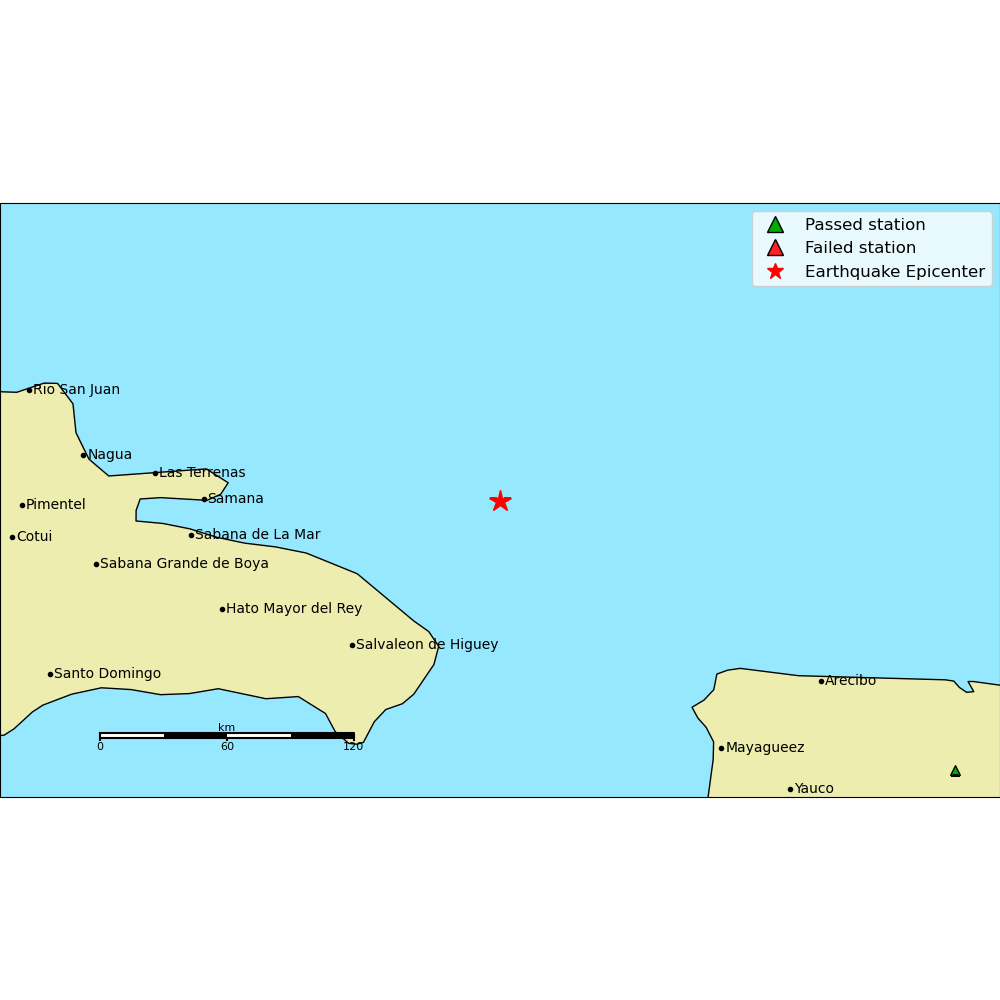
\includegraphics[width=0.9\textwidth]
    {stations_map.png}


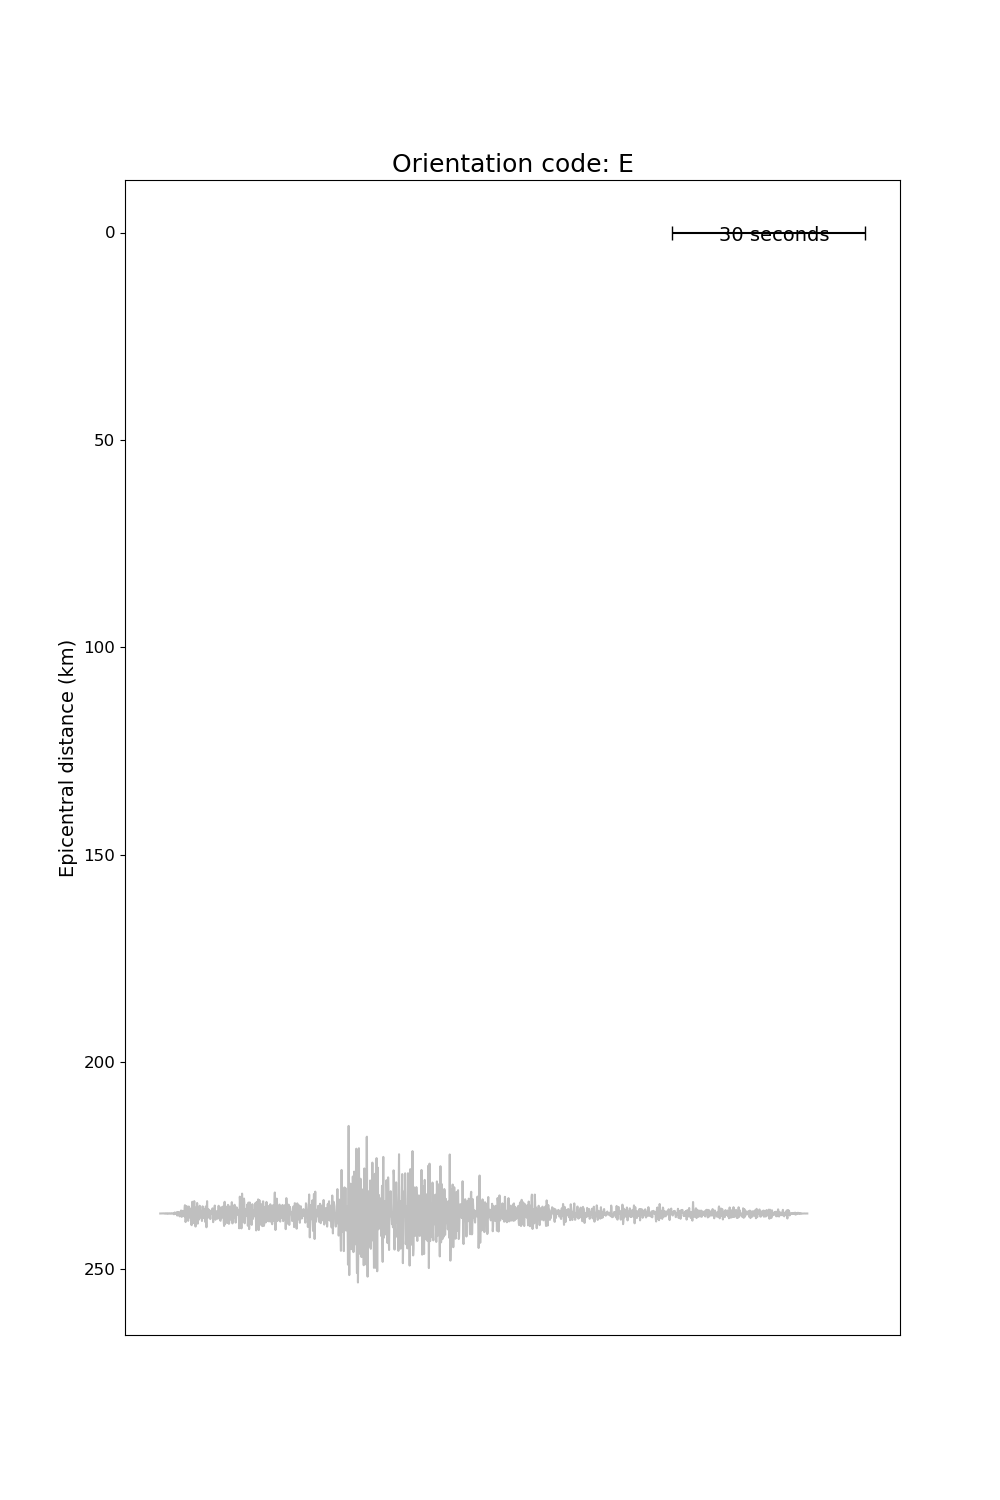
\includegraphics[width=0.9\textwidth]
    {moveout_plot.png}


\end{center}

\vfill

\newpage




\begin{tikzpicture}[remember picture,overlay]
   \draw[box] (0, 0.5) rectangle (9, 1.0) node[pos=.5]
       {\normalsize M 4.6 - 19931108034521 - 11/08/1993 03:45:20};
   \draw[box] (10, 0.5) rectangle (17, 1.0) node[pos=.5]
       {\normalsize IU.SJG.BH};
\end{tikzpicture}

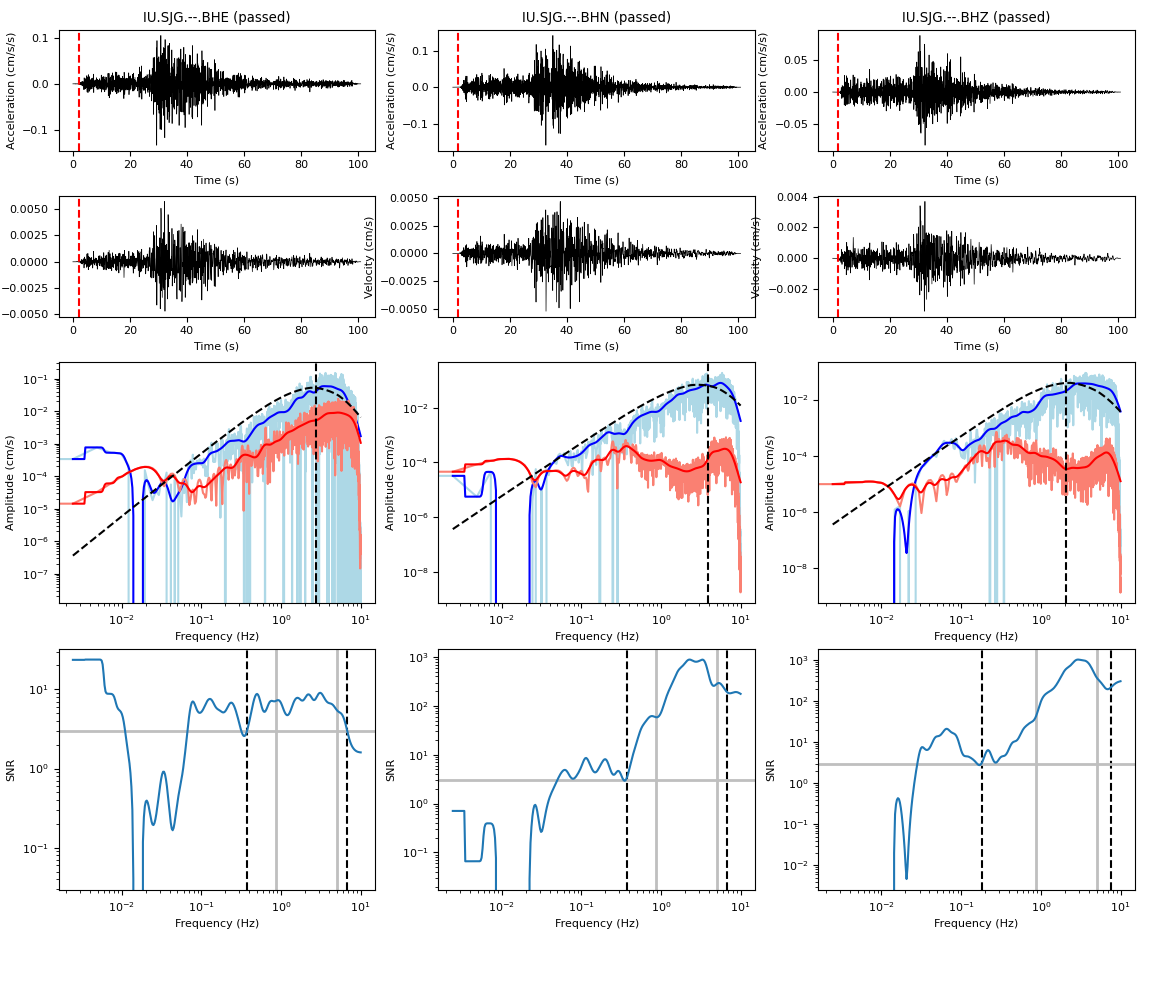
\includegraphics[height=5.75in]
    {plots/19931108034521_IU.SJG.BH.png}


\tiny
\begin{tabular}{lllll}
\toprule
    Process Step &  Process Attribute &            BHE Value &            BHN Value &            BHZ Value \\
\midrule
         Detrend &  detrending\_method &               demean &               demean &               demean \\
 Remove Response &        input\_units &               counts &               counts &               counts \\
                 &             method &      remove\_response &      remove\_response &      remove\_response \\
                 &       output\_units &               cm/s\textasciicircum 2 &               cm/s\textasciicircum 2 &               cm/s\textasciicircum 2 \\
         Detrend &  detrending\_method &               linear &               linear &               linear \\
         Detrend &  detrending\_method &               demean &               demean &               demean \\
             Cut &       new\_end\_time &  1993-11-08 03:47:35 &  1993-11-08 03:47:35 &  1993-11-08 03:47:35 \\
                 &     new\_start\_time &  1993-11-08 03:45:54 &  1993-11-08 03:45:54 &  1993-11-08 03:45:54 \\
           Taper &               side &                 both &                 both &                 both \\
                 &        taper\_width &                 0.05 &                 0.05 &                 0.05 \\
                 &        window\_type &                 Hann &                 Hann &                 Hann \\
 Highpass Filter &   corner\_frequency &       0.379435901373 &       0.379435901373 &       0.184530103348 \\
                 &       filter\_order &                    5 &                    5 &                    5 \\
                 &        filter\_type &          Butterworth &          Butterworth &          Butterworth \\
                 &   number\_of\_passes &                    2 &                    2 &                    2 \\
  Lowpass Filter &   corner\_frequency &        6.78302163724 &        6.78302163724 &                  7.5 \\
                 &       filter\_order &                    5 &                    5 &                    5 \\
                 &        filter\_type &          Butterworth &          Butterworth &          Butterworth \\
                 &   number\_of\_passes &                    2 &                    2 &                    2 \\
\bottomrule
\end{tabular}

Pick Method: travel\_time

\newpage


\end{document}
